\graphicspath{{chapters/04/}}
\chapter{Single cell multimodal omics}

All bulk omics are reaching a single-cell resolution, currently with
variable degrees of success. Some examples of trans-omics encompass
genome, transcriptome, proteome and metabolome. For instance,
single-cell applies both to \emph{epigenetic} (DNA and histone
modifications) and \emph{epitranscriptomics} (the ensemble of all RNA
modifications).

Single cell multimodal omics was classified as method of the year 2019
by Nature.

\hypertarget{single-cell-multiomic-profiling}{%
\subsection{Single-cell multiomic
profiling}\label{single-cell-multiomic-profiling}}

Linking measurements from different omics layers has the potential to
reveal regulatory and functional mechanisms underlying cell behaviour in
healthy development and disease. In Figure 4.1, we can observe the
possible connections among omics techniques and their interplay in
determining cell phenotype and functional potential as well as molecular
cell identity.

\begin{figure}
\centering
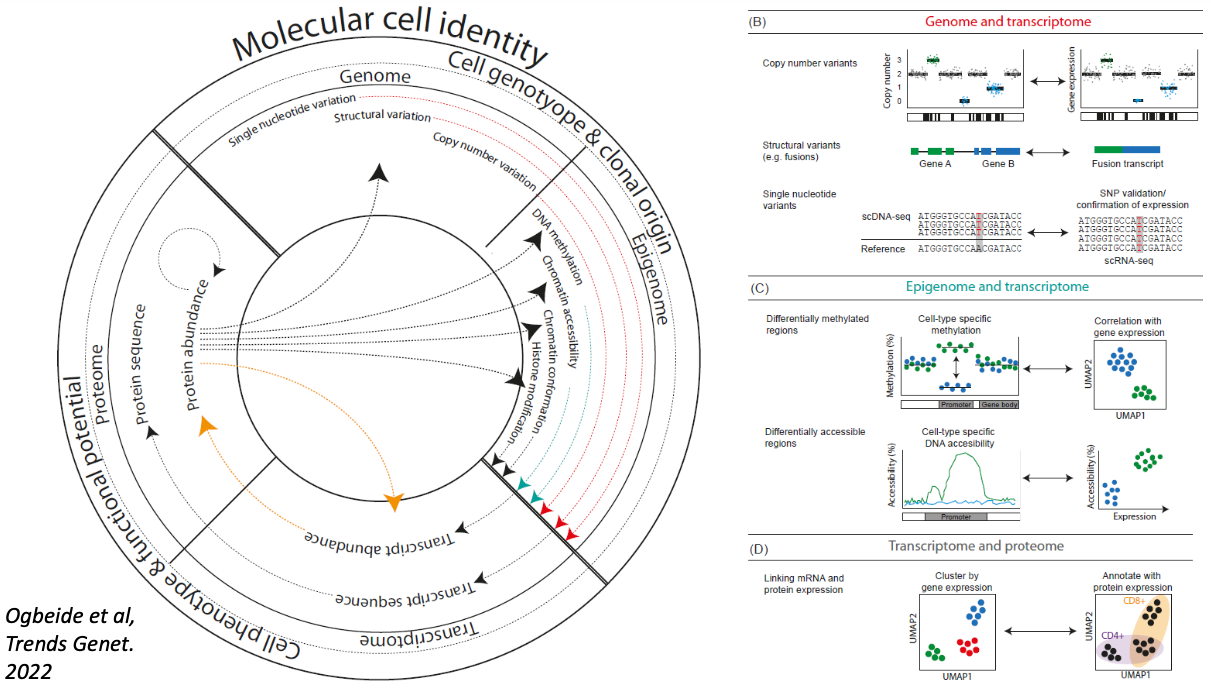
\includegraphics[width=0.5\textwidth]{images/Screenshot.png}
\caption{}
\end{figure}

\hypertarget{transcriptome-proteome}{%
\section{Transcriptome \& proteome}\label{transcriptome-proteome}}

Proteins determine much of cell behaviour and mRNA expression levels are
a weak proxy of protein expression (post-transcriptional and translation
regulation). In addition, there is no method for protein sequence
amplification (measurements are dependent on antibody-based detection or
mass spectrometry).

\hypertarget{cite-seq-cellular-indexing-of-transcriptomes-and-epitopes-2017}{%
\subsection{CITE-seq (Cellular Indexing of Transcriptomes and Epitopes)
(2017)}\label{cite-seq-cellular-indexing-of-transcriptomes-and-epitopes-2017}}

CITE-seq uses \textbf{DNA-barcoded antibodies} to convert detection of proteins
into a quantitative, sequenceable readout. Antibody-bound oligos act as
synthetic transcripts that are captured during most large-scale oligo
dT-based scRNA-seq library preparation protocols (e.g.~10x, Drop-seq). Cells labelled with panels
of antibodies, each tagged with a specific ADT (antibody derived tag),  are \textbf{captured in
parallel with the mRNA from the same cell} following lysis.

\begin{figure}
\centering
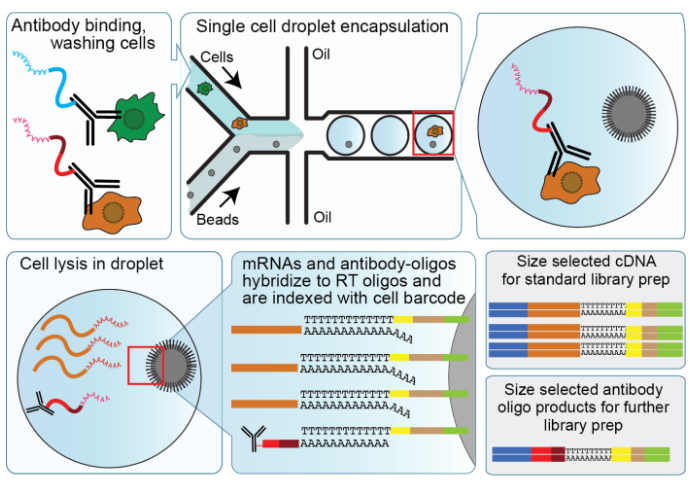
\includegraphics[width=0.5\textwidth]{images/Screen_Shot_2023-02-22_at_20-37-02.png}
\caption{cite-seq.com}
\end{figure}

\textbf{Pros:} immuno-phenotyping of cells allows a potentially
limitless number of markers unbiased transcriptome analysis.

\textbf{Cons:} specific antibodies necessary, for surface protein
markers

\hypertarget{cell-hashing-with-barcoded-antibodies}{%
\subsection{Cell Hashing with barcoded
antibodies (2018) }\label{cell-hashing-with-barcoded-antibodies}}

Oligo-tagged antibodies against \textbf{ubiquitously expressed} surface
proteins. Label cells from distinct samples, which can be \textbf{pooled}
(cost reduction). \textbf{Detection of doublets} between samples (or
within a sample, if used without pooling).

Other techniques based on barcoded antibodies:

\begin{itemize}
\tightlist
\item
  2017: \textbf{REAP-seq} (RNA Expression and Protein Sequencing assay).
  Peterson et al.~Nature biotechnology (library of 82 barcoded
  antibodies)
\item
  2017: \textbf{Abseq} (Ultrahigh- throughput single cell protein
  profiling with droplet microfluidic barcoding). Shahi et al,
  Scientific reports (example with 2 antibodies, B cells vs T cells)
\end{itemize}

\hypertarget{single-cell-mass-spectrometry-approaches-proteome-only}{%
\subsection{Single-cell mass-spectrometry approaches (proteome
only)}\label{single-cell-mass-spectrometry-approaches-proteome-only}}

Single cells are isolated in individual wells and lysed. Proteins
are digested to peptides. Peptides from each single cell are
\textbf{covalently labeled} (barcoded) with isobaric tandem-mass-tags
(TMT).

\begin{figure}
\centering
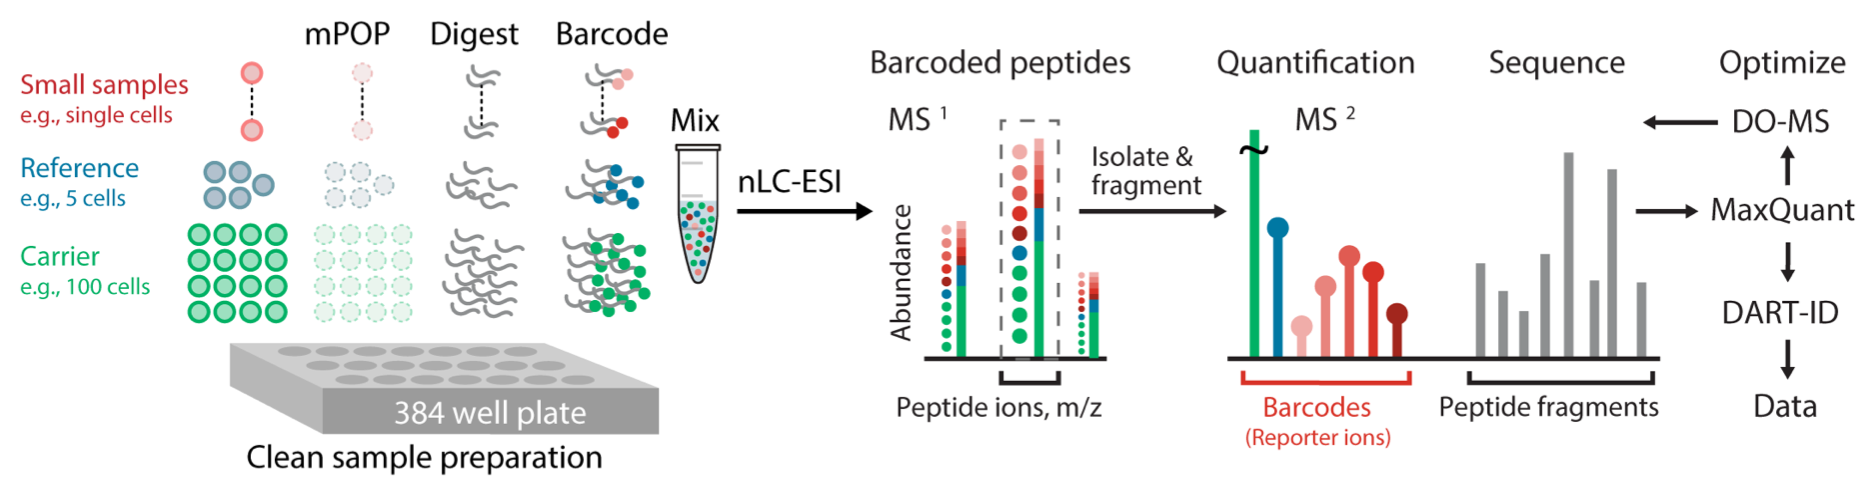
\includegraphics[width=0.5\textwidth]{images/Screenshot_1.png}
\caption{\emph{Specht et al, Genome Biology 2021}}
\end{figure}


SCoPE2 was applied to monocytes differentiated into macrophages.
Quantified over 3042 proteins in 1490 single monocytes and macrophages
in ten days of instrument time.

\hypertarget{transcriptome-genome}{%
\section{Transcriptome \& genome}\label{transcriptome-genome}}

Somatic variation is the genomic diversification between cells,
deviating from the ``original'' genome of the zygote. Somatic variation
can be:

\begin{itemize}
\tightlist
\item
  \emph{programmed}: during the maturation of lymphocytes, programmed
  rearrangements in B and T cell receptors are carried out
  e.g.~rearrangements of the V(D)J regions in B and T lymphocytes to
  produce diverse and specific antibodies and T cell receptors.
\item
  \emph{spontaneous}: accumulations of SNVs or CNVs of chromosome
  regions during development and aging
\end{itemize}

Potentially pathogenic when variants confer a competitive advantage to
the cell, leading to clonal expansion and the formation of malignant or
cancerous clones.

\hypertarget{dr-seq-2015}{%
\subsection{DR-seq (2015)}\label{dr-seq-2015}}

DR-seq (gDNA-mRNA sequencing) is based on sequencing of genomic DNA and
messenger RNA from the same cell. There are two different strategies for
amplifying:

\begin{itemize}
\tightlist
\item
  PCR for gDNA amplification
\item
  mRNA specific second-strand synthesis (polyA selection, only the 3'
  end is sequenced)
\end{itemize}

Coverage depth in a single cell should be 2, if we see more is produced
by amplification - differently from RNA-seq. There is a positive
correlation between copy number levels and average expression of all
genes located in the region of interest e.g.~chromosome 8.

\begin{figure}
\centering
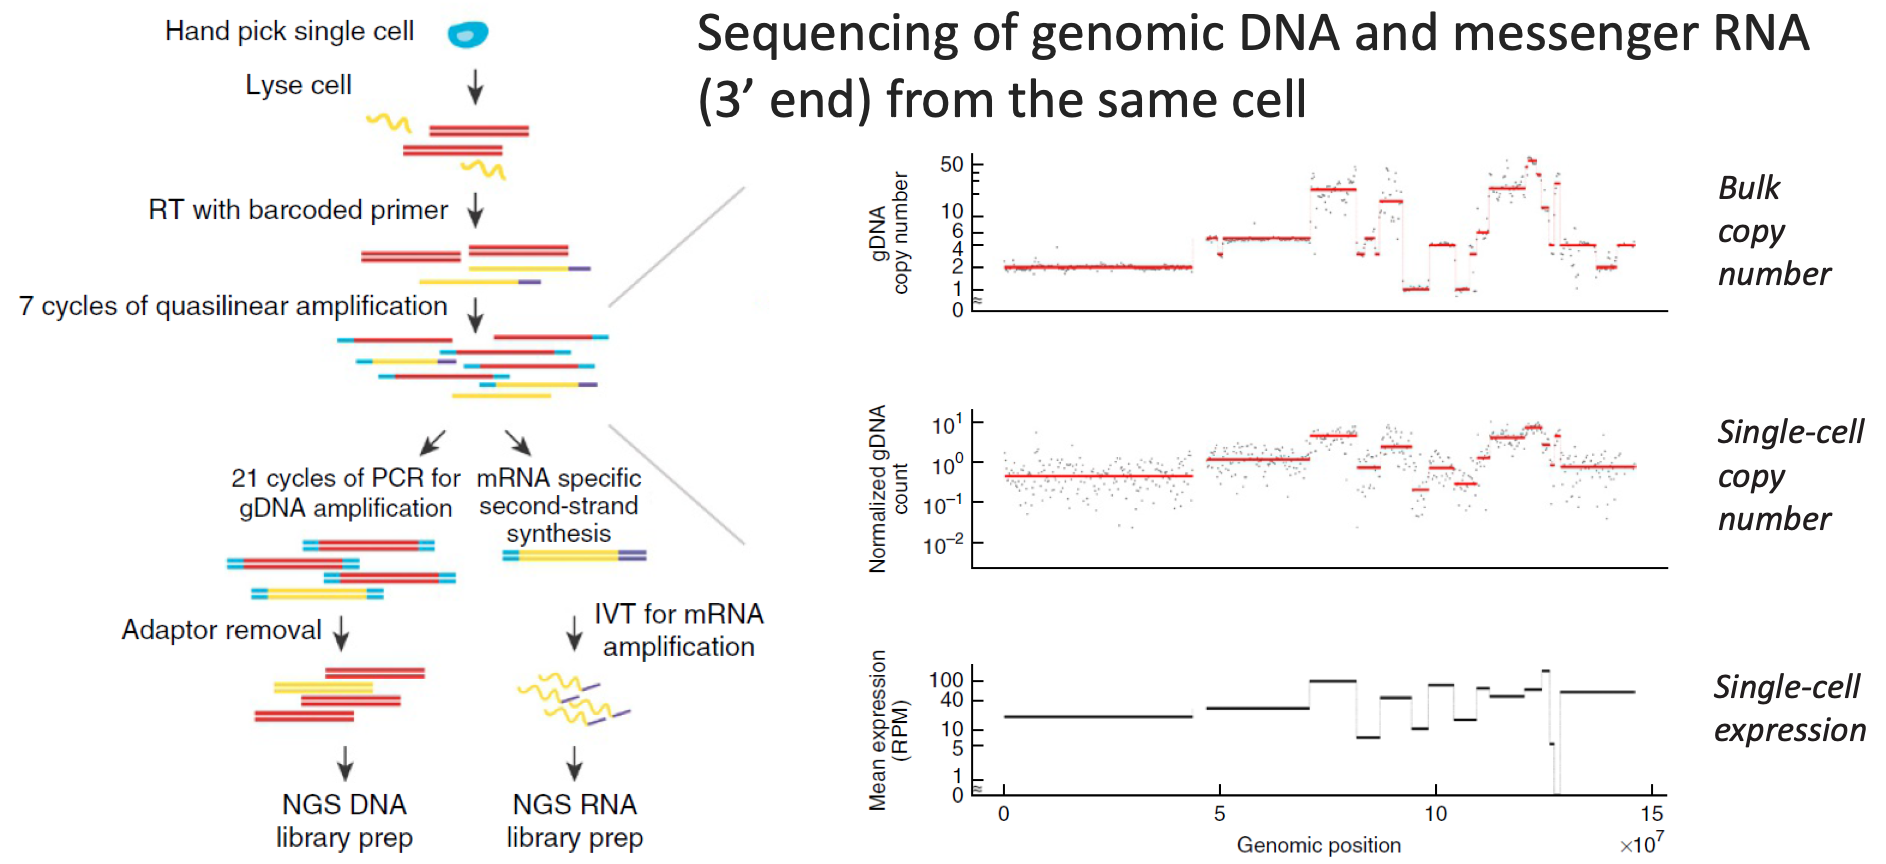
\includegraphics[width=0.5\textwidth]{images/Screenshot_2.png}
\caption{}
\end{figure}

\hypertarget{gt-seq}{%
\subsection{G\&T-seq}\label{gt-seq}}

Parallel sequencing of single-cell genomes and transcriptomes occurs
through physical separation of genomic DNA and poly(A)+ mRNA after cell
lysis, followed by separate amplification, library preparation and
sequencing. Full-length mRNA sequencing can be obtained following
Smart-seq2 protocol.

\textbf{Workflow:}

\begin{enumerate}
\def\labelenumi{\arabic{enumi}.}
\tightlist
\item
  isolate cells
\item
  lysis
\item
  using oligo-dT probes isolate mRNA content and divide it in different
  plates with respect to DNA

  \begin{enumerate}
  \def\labelenumii{\arabic{enumii}.}
  \tightlist
  \item
    RNA: whole transcriptome amplifications and full length sequencing
  \item
    DNA: whole genome amplification and detection
  \end{enumerate}
\end{enumerate}

The method was applied to differentiated neurons derived form trisomy 21
induced pluripotent stem cells and control disomy 21 iPSCs. By visual
inspection, we can clearly see a gain in chromosome 21 with respect to
control, even though some error is identified. The positive
result is that chromosome 21 genes are more expressed with respect to
control. Transcriptomics variation was also observed in other autosomes,
which could be due to both biological and technical variation.

\begin{figure}
\centering
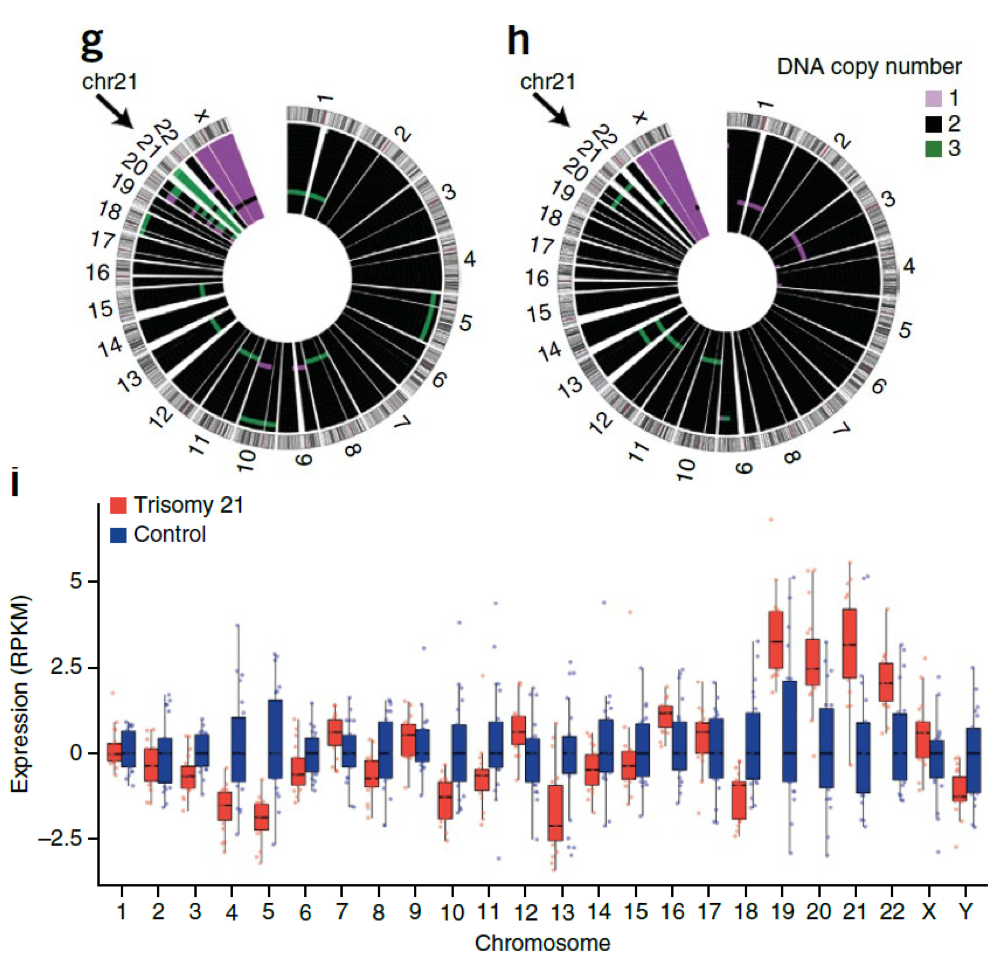
\includegraphics[width=0.5\textwidth]{images/Screenshot_3.png}
\caption{\emph{Macaulay et al, Nature Methods 2015}}
\end{figure}


In theory these approaches can be used to detect fusions, while SNVs are
harder to be found at low coverage. There could be location biases, but
this is common for different amplification techniques.

\hypertarget{physical-separation-of-the-nucleus-and-cytoplasm}{%
\subsection{Physical separation of the nucleus and
cytoplasm}\label{physical-separation-of-the-nucleus-and-cytoplasm}}

In this case there is no separation of DNA and RNA, but rather of the
nucleus (DNA-seq) and cytoplasm (RNA-seq). Cell separation is performed
by sorting, but the core of the technique a gentle lysis and separation
in two plates. Full length mRNA sequencing is comparable with
SMART-seq2, while for DNA tagmentation is performed.

\begin{figure}
\centering
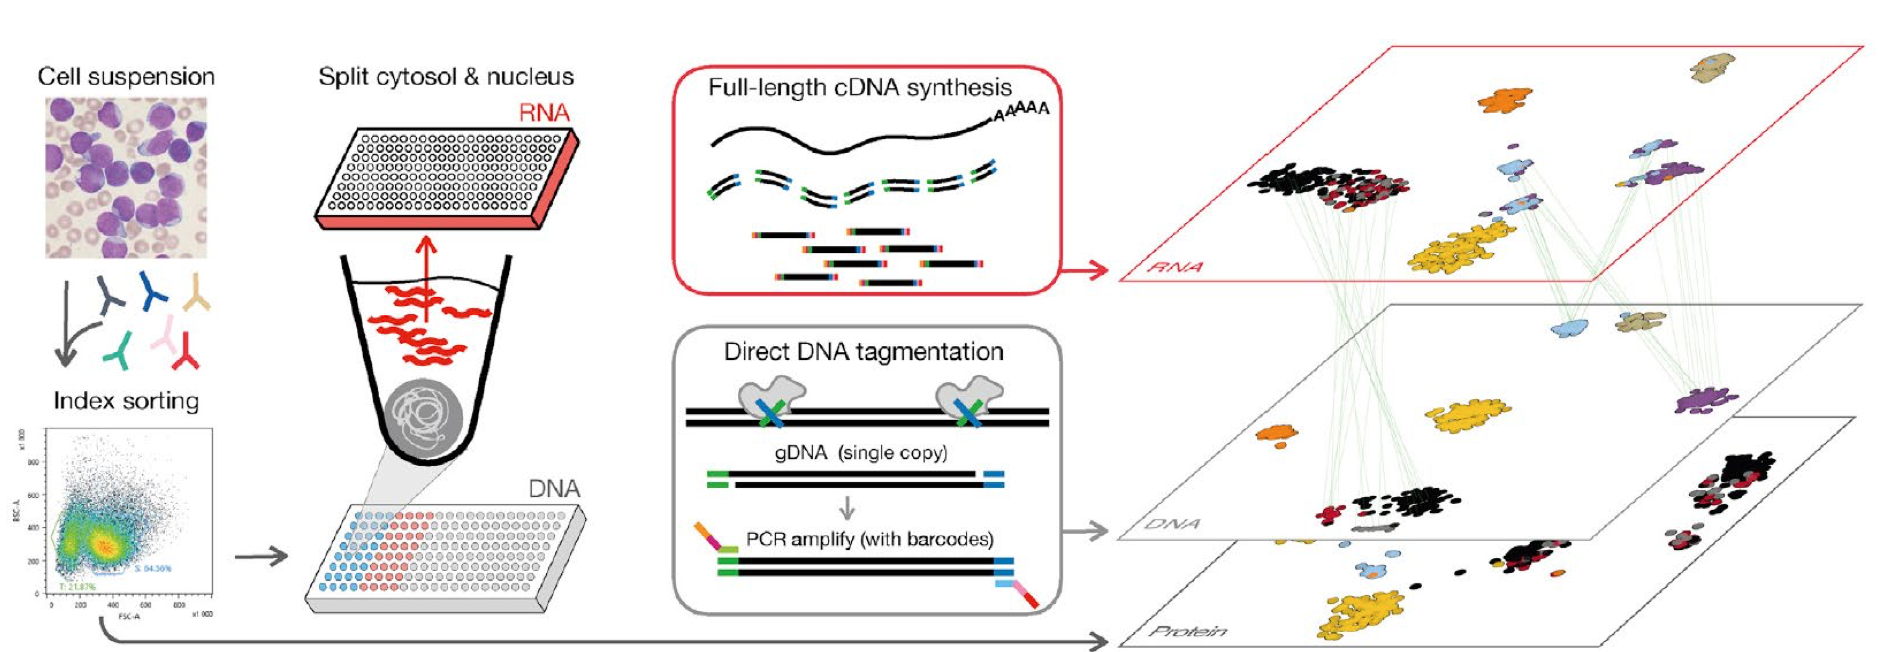
\includegraphics[width=0.5\textwidth]{images/Screenshot_4.png}
\caption{\emph{Zachariadis et al, Molecular Cell 2020}}
\end{figure}

\hypertarget{genotyping-of-transcriptomes-got-2019}{%
\subsection{Genotyping of Transcriptomes (GoT)
(2019)}\label{genotyping-of-transcriptomes-got-2019}}

\begin{figure}
\centering
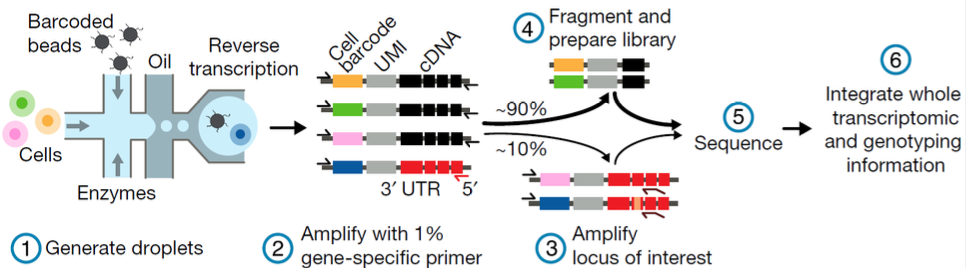
\includegraphics[width=0.5\textwidth]{images/Screen_Shot_2023-02-22_at_20-38-39.png}
\caption{\emph{Nam et al, Nature 2019}}
\end{figure}

GoT integrates \emph{genotyping} (detection of somatic mutations gene of
interest) with single cell RNA sequencing. The main advantage of this
technique is the identification of malignant cells associated with a
specific mutation(challenging in the absence of specific surface
markers). Additionally, this method works with droplet-based methods,
greatly enhancing the throughput.

We can connect the presence of a mutation with markers and cell
abundance. The real advantage is the amplification of the locus of
interest reducing the dropout rate.

\hypertarget{adaptive-immune-response}{%
\subsection{Adaptive immune response}\label{adaptive-immune-response}}

Both lymphocytes express B- and T-cell receptors. The soluble part in
both receptor is an antibody able to recognize antigens. The
transmembrane domain is common, while the top part is a variable region.
Looking at gDNA of each cell, we have a V(D)J region where random
stochastic rearrangement occur, producing variability in the amino acid
region of the receptor. Once one of these cells meets a pathogen, we
have the activation of the response and increase in antibody targeting a
specific antigen. Through the sequence of the VDJ region, we can
identify the abundance of the pathogen e.g.~COVID.

\begin{figure}
\centering
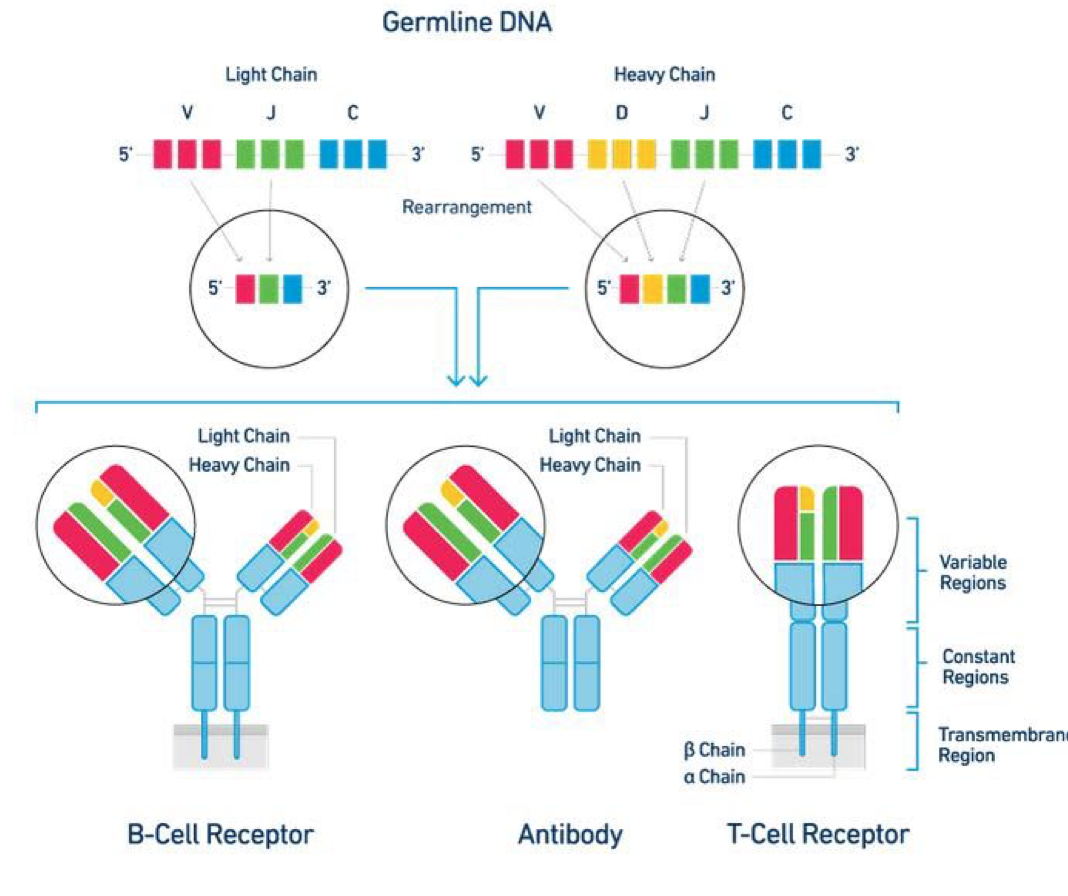
\includegraphics[width=0.5\textwidth]{images/Screenshot_5.png}
\caption{\emph{https://www.10xgenomics.com}}
\end{figure}


\hypertarget{immune-profiling-protocol}{%
\subsubsection{Immune profiling
protocol}\label{immune-profiling-protocol}}

The most used platform (10x) has an \textbf{immune profiling protocol}
implementing this technique through transcriptome 5' end sequencing for
paired T- and B-cell receptors. After barcoding, libraries are split for
the targeted analysis of B/T cell receptor transcripts, (based on
primers specific for the sequence of the constant region) and the
analysis of all other transcripts (standard 10x 5' sequencing).

Sequencing of TCR alpha and beta chain allows cell grouping according to
shared sequences. It is possible to predict the pathogen to which the
receptor will react e.g.~the clonal expansion is recognizing a sequence
of a particular peptide of cytomegalovirus.

\hypertarget{transcriptome-epigenome}{%
\section{Transcriptome \& epigenome}\label{transcriptome-epigenome}}

The compactness of DNA is regulated by protein modifications that act on
chromatin accessibility and therefore have an effect on gene
transcription. Epigenetic modifications contribute to cellular
heterogeneity and regulation of gene expression during development,
lineage determination and response to dynamic stimuli. In single cell
epigenomics we can study:

\begin{itemize}
\tightlist
\item
  DNA methylation
\item
  chromatin accessibilty
\end{itemize}

\hypertarget{dna-methylation}{%
\subsection{DNA methylation}\label{dna-methylation}}

DNA methylation was the first discovered epigenetic mark, which consists
on an addition of a methyl group on cytosine residues of the
dinucleotide \textbf{CpG.} Methylation is implicated in repression of
transcriptional activity. \textbf{Bisulphite sequencing} is a technique
based on treating DNA with sodium bisulphite, which allows the
conversion of cytosines to uraciles through alkylation in the case of
unmethylated cytosine - while methylated cytosine will remain unchanged.
By analyzing mismatches with a reference genome sequence, we can
distinguish methylated from unmethylated cytosines.

\hypertarget{scmt-seq-2016}{%
\subsubsection{scM\&T-seq (2016)}\label{scmt-seq-2016}}

Single-cell methylome \& transcriptome is a derivation of G\&T-seq,
based on the physical separation of DNA and RNA:

\begin{itemize}
\tightlist
\item
  Smart-seq2 on mRNA
\item
  Bisulphite sequencing on DNA
\end{itemize}

The technique was applied to mouse embryonic stem cells in the first
publication of the technique. Several single cell genome and
transcriptome methods can be extended to study the methylome by applying
bisulphite sequencing.

\begin{figure}
\centering
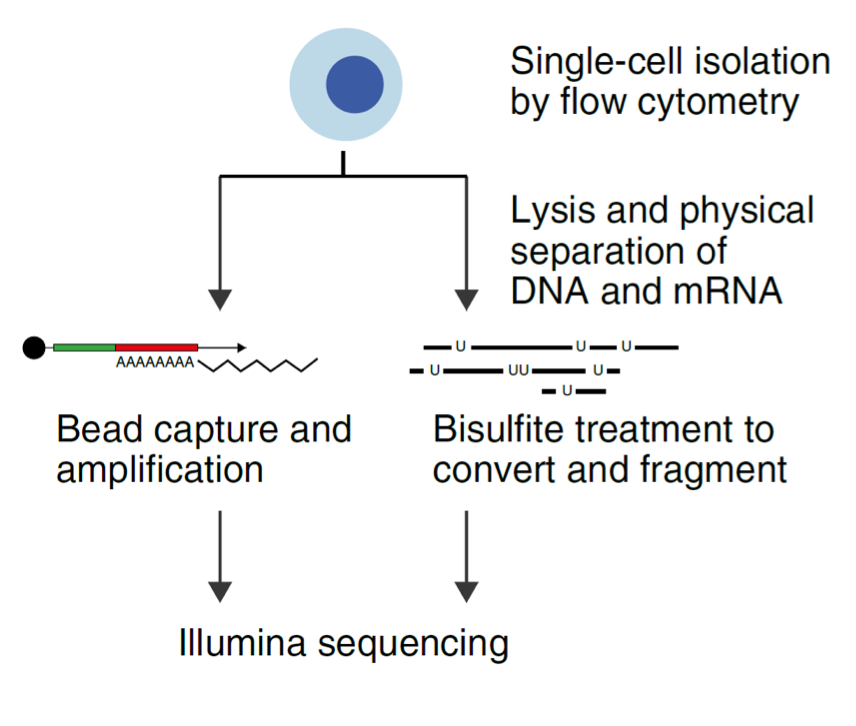
\includegraphics[width=0.5\textwidth]{images/Screenshot_6.png}
\caption{\emph{Angermueller et al, Nature Methods 2016}}
\end{figure}

\hypertarget{chromatin-accessibility}{%
\subsection{Chromatin accessibility}\label{chromatin-accessibility}}

\hypertarget{atac-seq-2013}{%
\subsubsection{ATAC-seq (2013)}\label{atac-seq-2013}}

ATAC-seq (Assay for Transposable Accessible Chromatin) is designed to
identify open chromatin regions in the genome by high-throughput
sequencing. The technique is based on the activity of a key enzyme,
\textbf{Tn5 Transposase}, which performs a ``cut and paste'' procedure
and can be engineered into a hyperactive mutant form. Tn5 transposases
preferentially insert into open chromatin sites, cut and add two
sequencing primers (t\emph{agmentation}). The obtained fragments will be
nucleosome free or nucleosome containing. The technique is very
sensitive i.e.~works with small amounts of material and faster than
alternative methods.

\begin{figure}
\centering
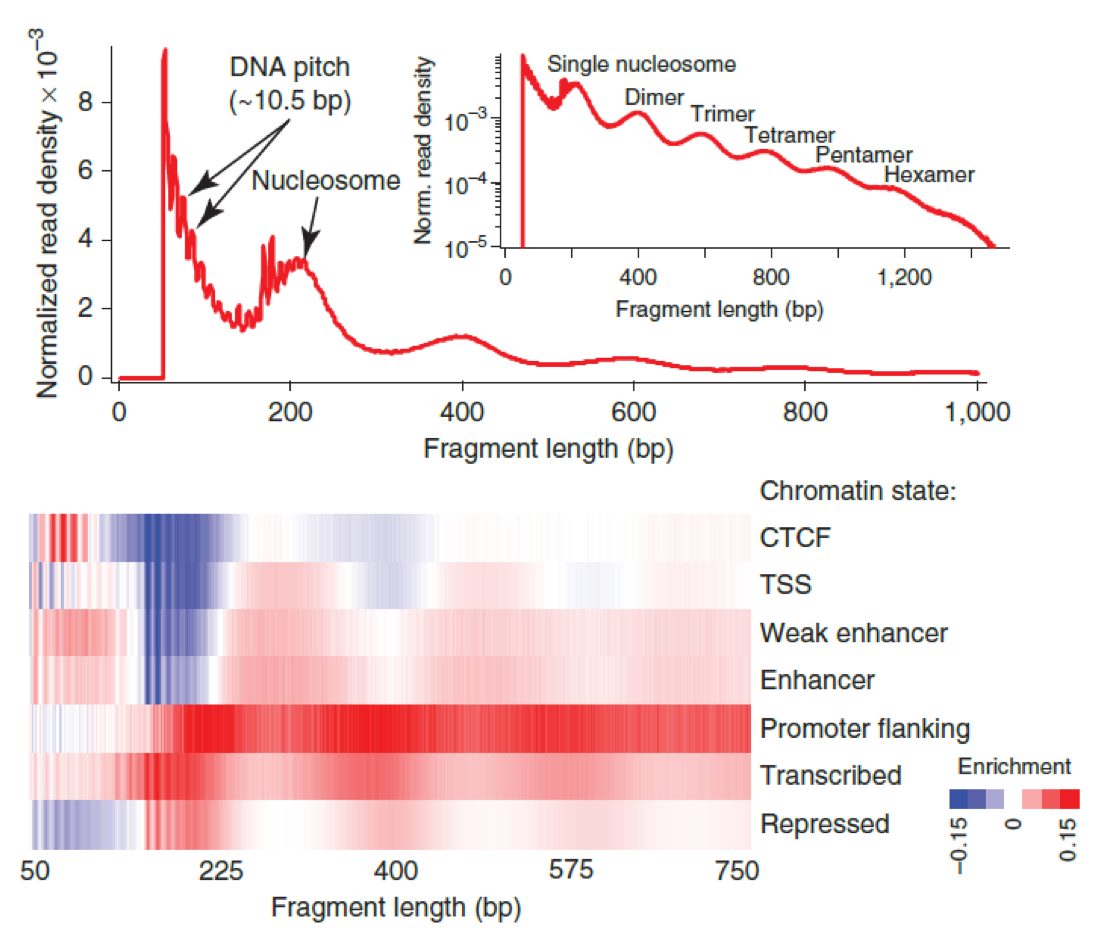
\includegraphics[width=0.5\textwidth]{images/Screenshot_7.png}
\caption{\emph{Buenrostro et al, Nature Methods 2013}}
\end{figure}

\textbf{Key features to identify a successful ATAC-seq experiment}:

\begin{itemize}
\tightlist
\item
  fragment size peaks should follow a clear periodicity of
  \textasciitilde200 bp length, corresponding to multiples of
  nucleosome-wrapped sequence size
\item
  at the genome-wide level, fragments will be enriched in open chromatin
  regions:

  \begin{itemize}
  \tightlist
  \item
    promoter flanking regions
  \item
    transcribed genes
  \end{itemize}
\end{itemize}

\hypertarget{single-cell-atac-seq-2015}{%
\subsubsection{Single cell ATAC-seq
(2015)}\label{single-cell-atac-seq-2015}}

ATAC-seq was adapted to single cell resolution with a fluidigm device
(not yet droplet-based, lower throughput). We can analyze a snapshot of
a genome portion comparing fragment peaks generated from bulk ATAC-seq
to aggregate single cell ATAC-seq peaks (obtained from 254 cells) and
verify that there is a high correlation among peaks, which are located
close to the TSS. It is possible to map fragments on a single cell
profile, which will have a range from 0 to 2 fragments per position. The
protocol can be adapted to any single cell approach e.g.~droplet-based
or combinatorial indexing. In 2018, 10x developed 10x single-cell
ATAC-seq with a similar workflow; the main difference is the usage of
nuclei instead of cells and the capture procedure without UMI (directly
designed for transposase adapters).

``Why always chromosome 19?''

\begin{figure}
\centering
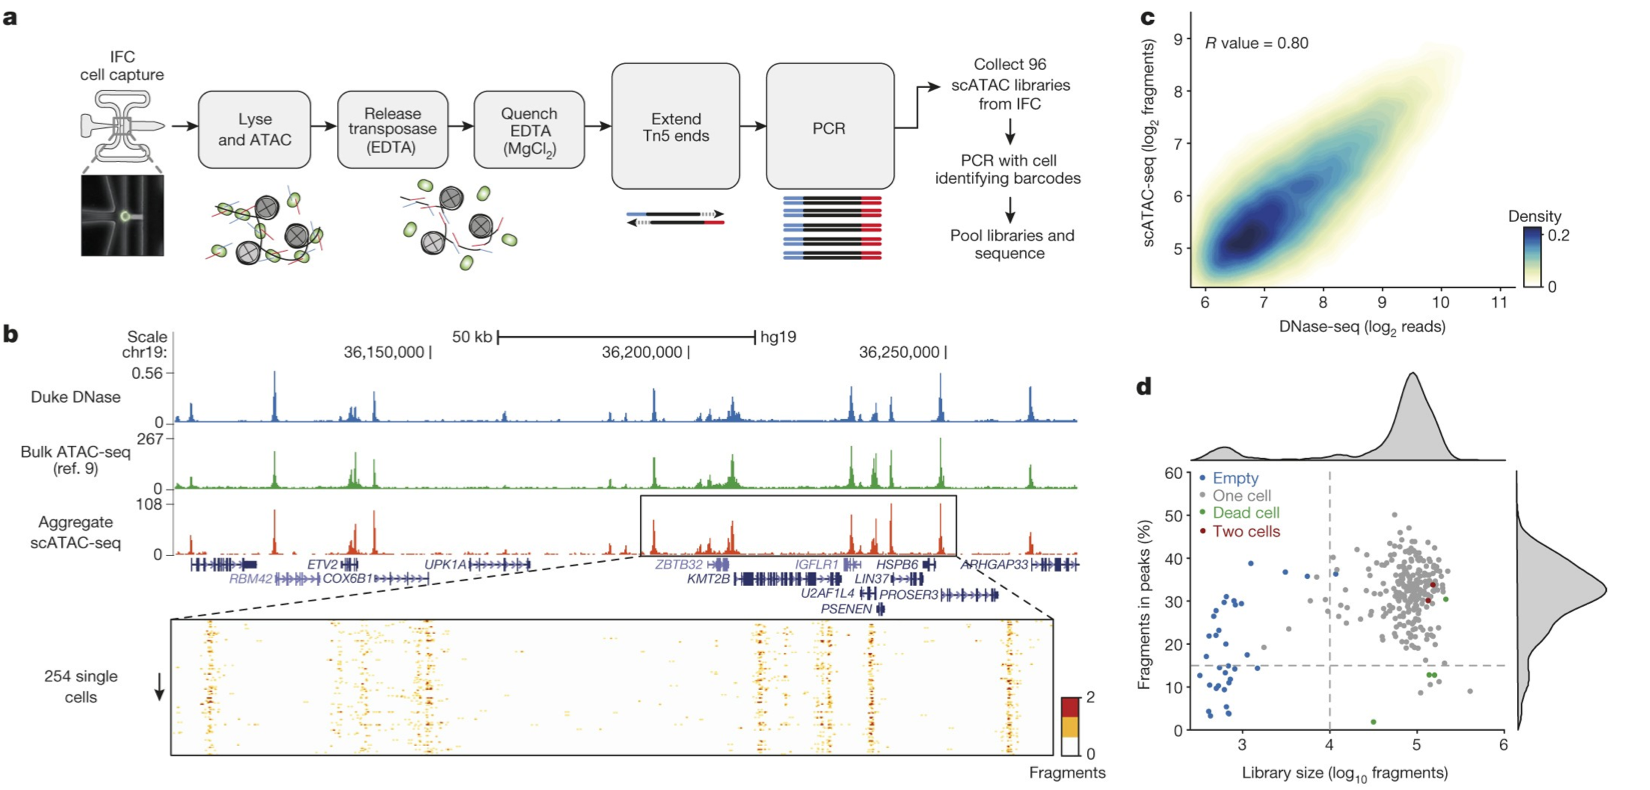
\includegraphics[width=0.5\textwidth]{images/Screenshot_8.png}
\caption{\emph{Buenrostro et al, Nature 2015}}
\end{figure}


\hypertarget{peak-calling}{%
\subsubsection{Peak calling}\label{peak-calling}}

In order to reduce the dimensions, one of the first steps in the
analysis is peak calling, which can be performed by Cell Ranger on 10x
data. The number of transpositions events is evaluated in pseudo-bulk,
followed by a smoothing procedure and signal threshold evaluation to
discriminate actual signal from noise e.g.~zero negative binomial model.
The outputs of this step are:

\begin{enumerate}
\def\labelenumi{\arabic{enumi}.}
\tightlist
\item
  indexed fragment file collecting all the reads, even if they do not
  map to a peak, which can be used for quality control.
\item
  large sparse matrix, where each row is a genomic range corresponding
  to a peak and the column the number of fragments per cell
\end{enumerate}

The main challenges in comparison to scRNA are:

\begin{itemize}
\tightlist
\item
  more sparse data
\item
  near-binary data (open vs closed, we are not really interested on how
  much)
\item
  non-fixed feature set (variable features according to number of peaks
  per cell)
\item
  order of magnitude more features
\end{itemize}

\hypertarget{enrichment}{%
\subsubsection{Enrichment}\label{enrichment}}

After peak calling, it is possible to perform DNA sequence enrichment on
motif to identify transcription factor binding sites. Regulatory
relationship among enhancers and promoters can be studied through
co-accessibility networks and gene variants can be studied through
genetic variant enrichment.

While working with Seurat, the best approach is to apply
\textbf{Signac}, a Seurat extension for the analysis of ATAC-seq data.

\hypertarget{snare-seq-2019}{%
\subsection{SNARE-seq (2019)}\label{snare-seq-2019}}

Single-Nucleus chromatin Accessibility and mRNA Expression is a
high-throughput sequencing of the transcriptome and chromatin
accessibility in the same nucleus. In this setting, there is no need for
probabilistic mapping of single-cell clusters from separate analyses.
The technique was applied to droplet-based method, then adopted by 10x
(Multiome profiling).

Capturing beads contain two adapters, one for ployA selection for mRNA
and another complementary to Tn5. The advantage is that probes have the
same barcode, allowing easy mapping of both libraries and digital
counting matrix with common columns.

\begin{figure}
\centering
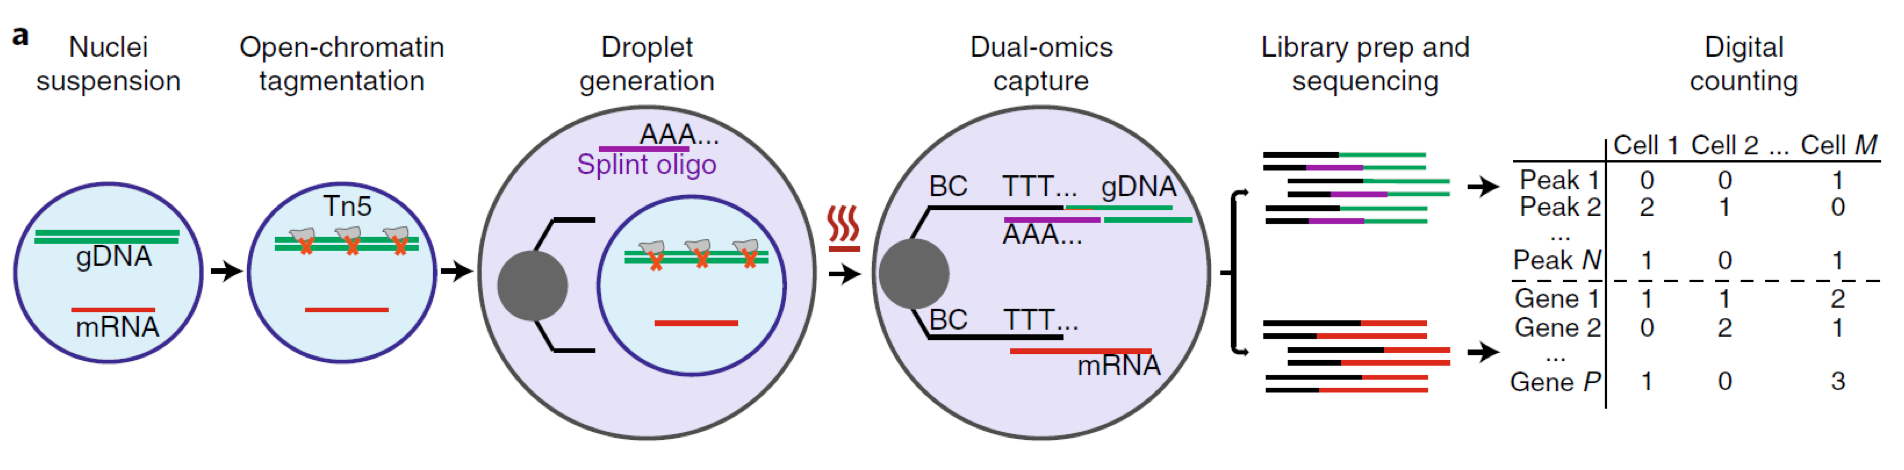
\includegraphics[width=0.5\textwidth]{images/Screenshot_9.png}
\caption{Chen et al, Nature Biotechnology 2019}
\end{figure}


In the original publication the method was applied to
\textasciitilde5000 nuclei from 5 mice collected from neonatal cerebral
cortex. The clusters have been annotated to known groups of neuronal
cells based on gene expression (reference) and then mapped to the UMAP
obtained from chromatin data analysis. The obtained result is more or
less consistent with the expectation and allows the study of biological
implications of chromatin regulation on gene expression. Alternatively,
it is possible to use both approaches simultaneously to identify
clusters.

\begin{figure}
\centering
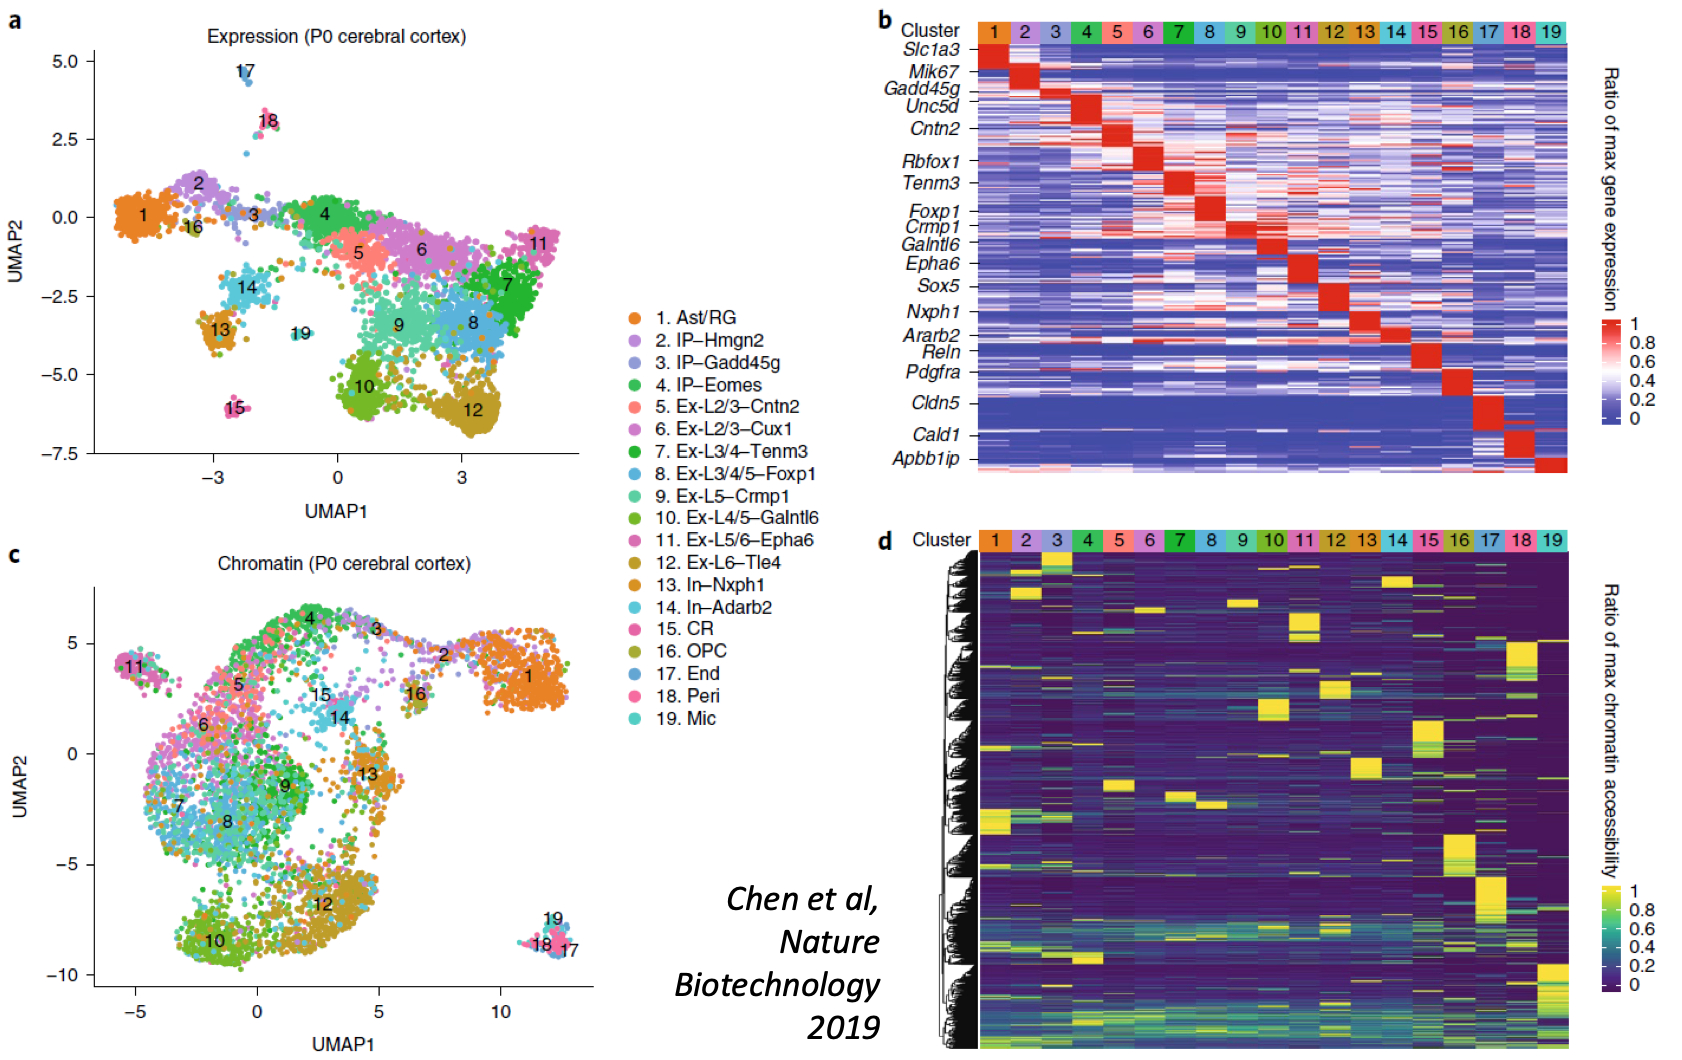
\includegraphics[width=0.5\textwidth]{images/Screenshot_10.png}
\caption{Chen et al, Nature Biotechnology 2019}
\end{figure}

10x method for simultaneous detection of gene expression and chromatin
state from the same cell can aid in identifying activation of gene
expression even though expression data does not show relevant patterns.
In addition, putative regulatory elements directly linked to a gene of
interest can be inferred thanks to the correlation of gene expression
with the presence of accessible peaks in clusters.

\begin{figure}
\centering
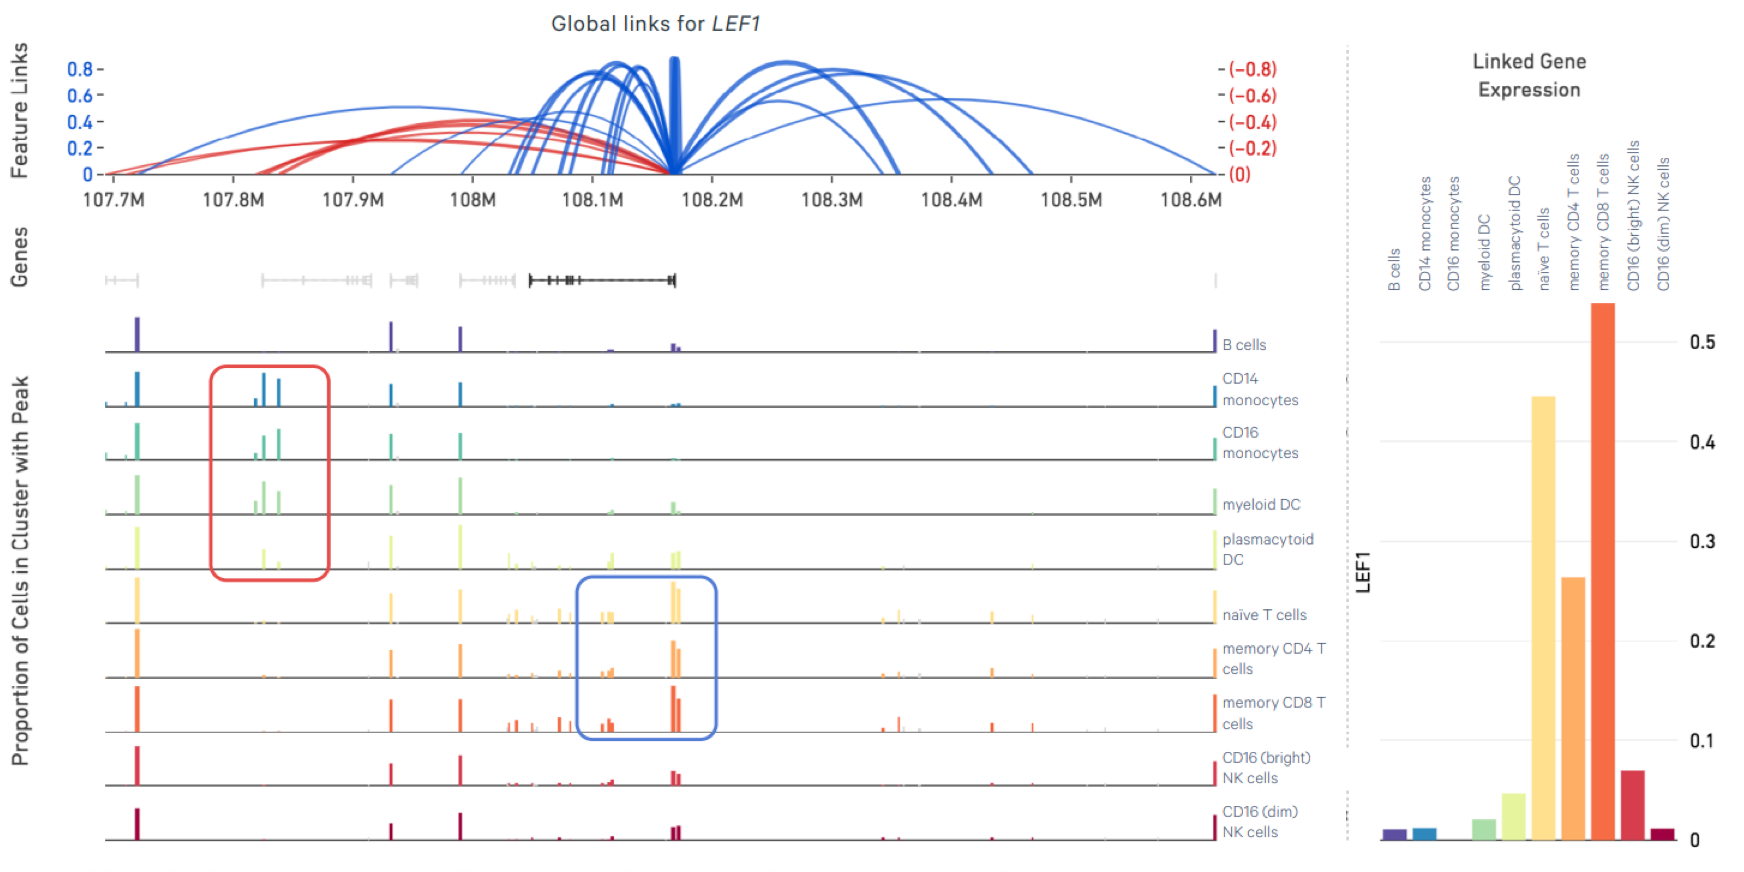
\includegraphics[width=0.5\textwidth]{images/Screenshot_11.png}
\caption{\emph{https://www.10xgenomics.com}}
\end{figure}

\hypertarget{transcriptome-crispr-perturbations}{%
\section{Transcriptome \& ``CRISPR''
perturbations}\label{transcriptome-crispr-perturbations}}

CRISPR technology can be applied to inactivate regions of interest and
study perturbation effects (also called \emph{reverse genetics}
approach).

\hypertarget{perturb-seq-2016}{%
\subsection{Perturb-seq (2016)}\label{perturb-seq-2016}}

Perturb-seq combines single-cell RNA sequencing with CRISPR- based
perturbations (inactivation of genes). The main aim is to map the
transcriptional effects of genetic perturbations and identify regulatory
circuits. By applying single cell, we can detect the expression level of
each cell and identify which kind of CRISPR guide was present in each
cell i.e.~which gene was inactivated.

\begin{figure}
\centering
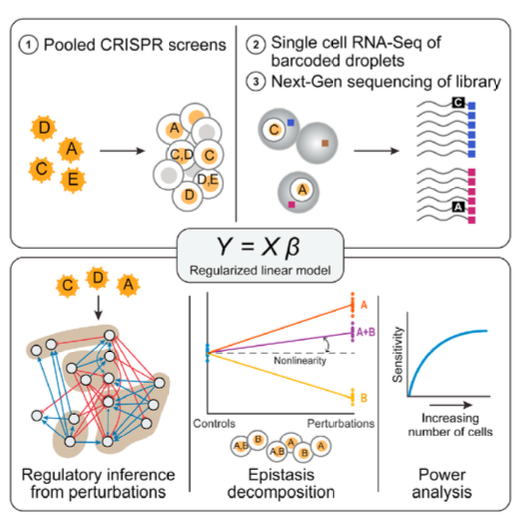
\includegraphics[width=0.5\textwidth]{images/Screen_Shot_2023-02-22_at_20-40-56.png}
\caption{Dixit et al, Cell 2016}
\end{figure}


The mRNAs are captured with a cell barcode (\textbf{CBC}) and matched to
sgRNAs and paired guide barcode (\textbf{GBC}).

\begin{figure}
\centering
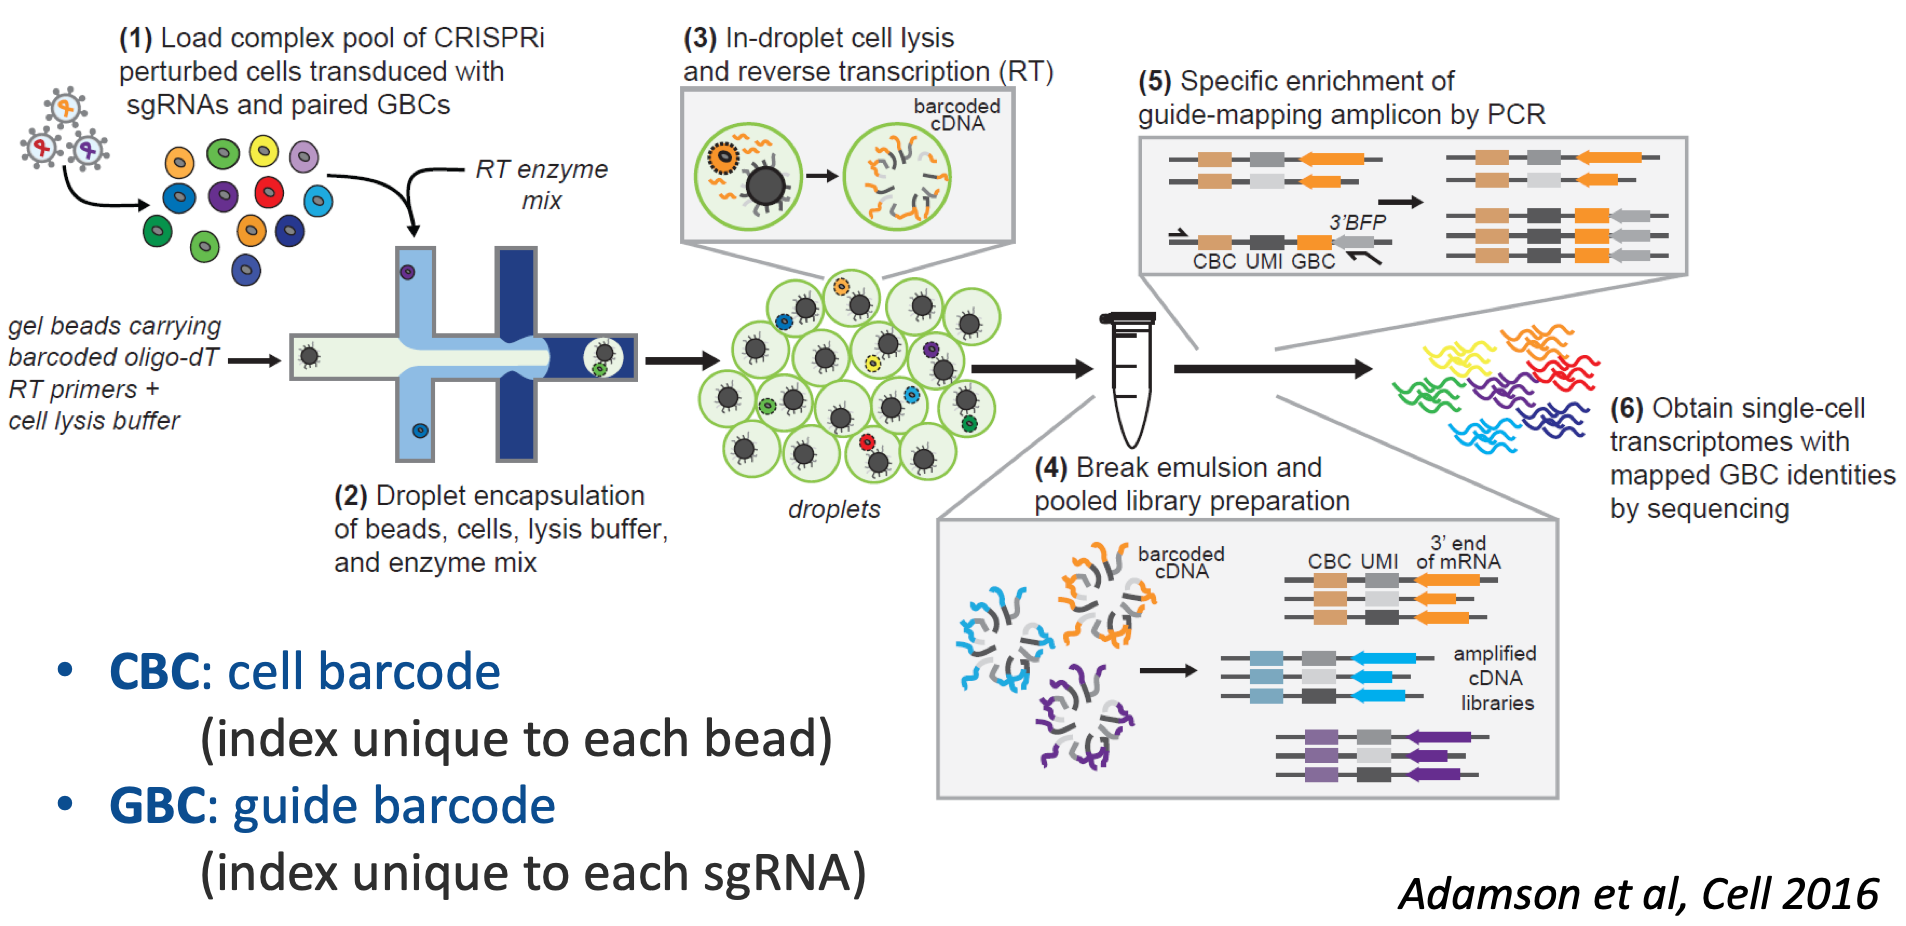
\includegraphics[width=0.5\textwidth]{images/Screenshot_12.png}
\caption{}
\end{figure}

\hypertarget{crisp-seq-2016}{%
\subsection{CRISP-seq (2016)}\label{crisp-seq-2016}}

CRISP-seq combines single-cell RNAseq with CRISPR-based perturbations
(editing/inactivation of genes). It allows to discover interactions and
redundancies between developmental and signaling- dependent factors. The
technique exploits mathematical modeling and immune stimulation factors.

\begin{figure}
\centering
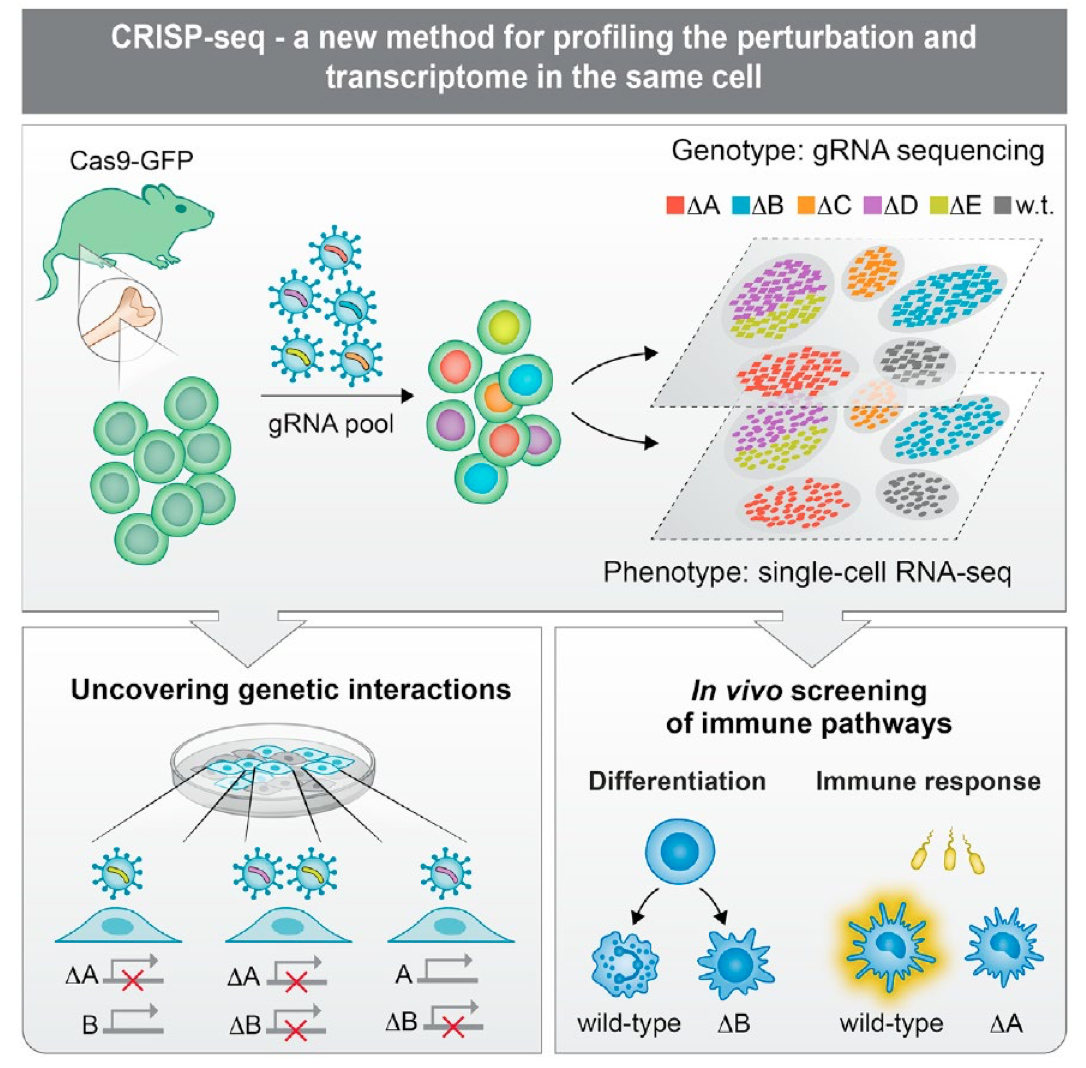
\includegraphics[width=0.5\textwidth]{images/Screenshot_13.png}
\caption{\emph{Jaitin et al, Cell 2016}}
\end{figure}

\hypertarget{x-crispr-screen}{%
\subsubsection{10x CRISPR screen}\label{x-crispr-screen}}

In addition, 10x now provides single-cell CRISPR screens, which provide
information on:

\begin{enumerate}
\def\labelenumi{\arabic{enumi}.}
\tightlist
\item
  guide RNAs
\item
  whole transcriptome profiling
\item
  cell surface protein expresssion
\item
  isolation of paired immune receptor sequences
\end{enumerate}

\hypertarget{challenges-and-opportunities-in-single-cell-multimodal-omics}{%
\section{Challenges and opportunities in single-cell multimodal
omics}\label{challenges-and-opportunities-in-single-cell-multimodal-omics}}

\begin{figure}
\centering
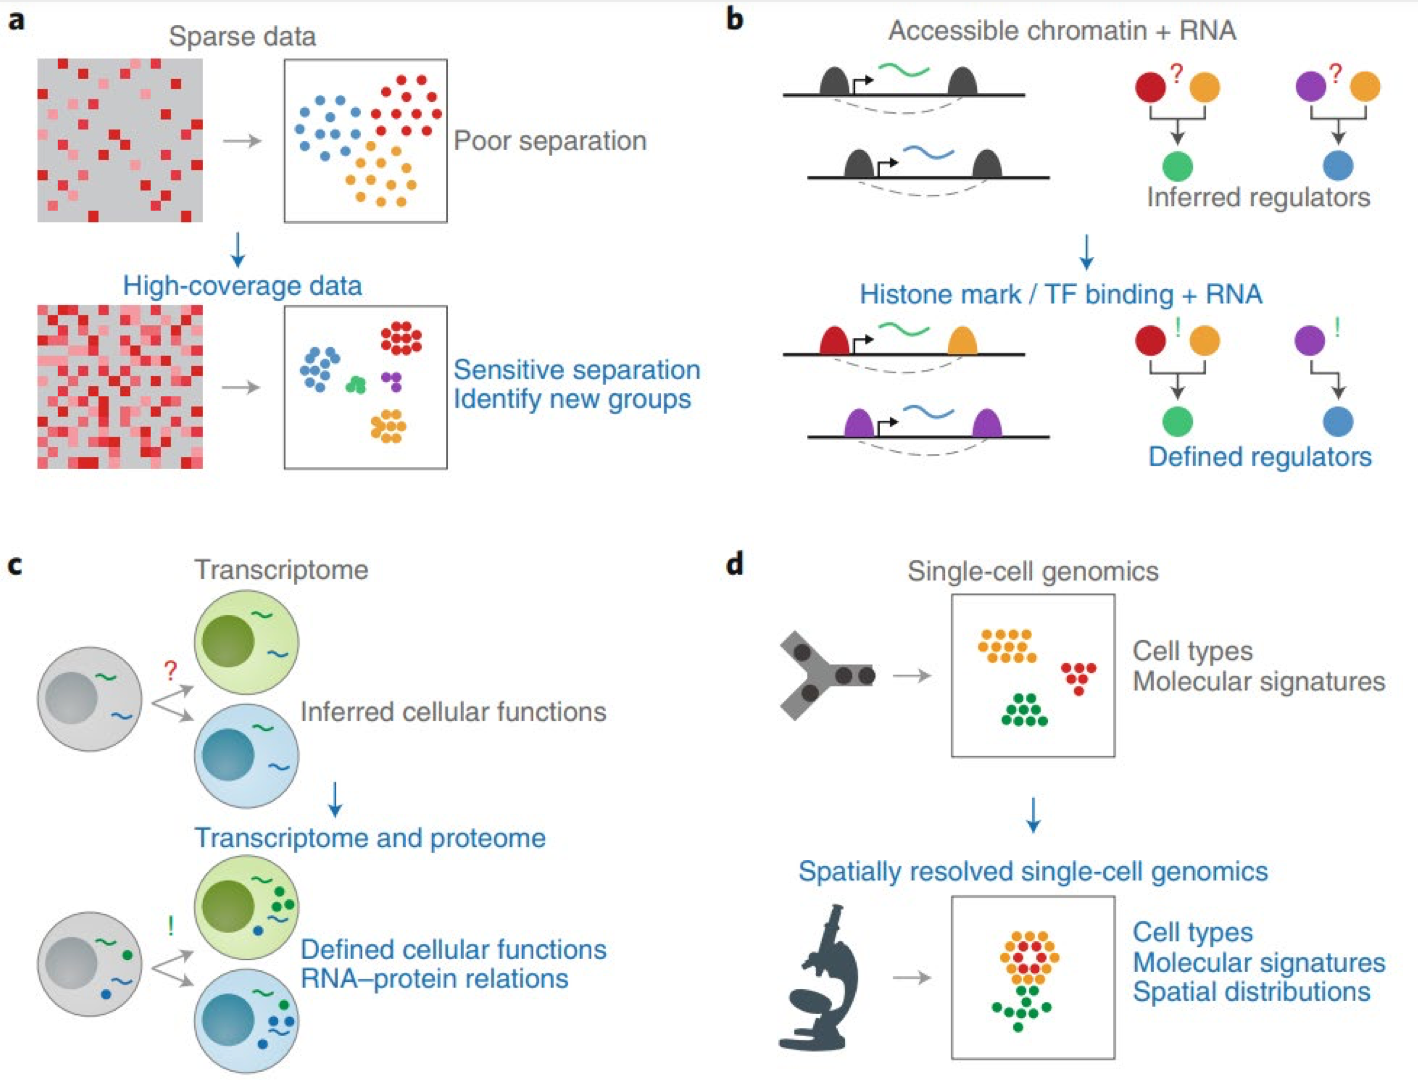
\includegraphics[width=0.5\textwidth]{images/Screenshot_14.png}
\caption{\emph{Zhu C et al.~Nat Methods. 2020}}
\end{figure}


Chromatin accessibility layer is more sparse than the genomic one, so
the combination of multiple layers can aid in achieving a better
separation. This instead in not an issue with tagged antibodies, but on
the other hand we are working with restricted information and mainly on
surface proteins. Epigenetic information on histone marks and TF
binding, even though not in the same cell, can be combined to study
regulatory networks.
